\section{Repetition/Introduction to Simulink/QuaRC}\label{sec:prob1}
%<<<<<<< HEAD

%=======
Simulink is a program for Model-Based Design. It overtakes the code from Matlab, compiles it into the C language and sends it to the right controllers. QuaRC\footnote{\url{http://www.quarcservice.com/ReleaseNotes/files/quarc_user_guide.html}} is a Real-Time control system, that is integrated into Simulink. To control the program, Matlab and Simulink is used. We use QuaRC for the build option as can be shown on figure \ref{fig:simDiag}. 
The work flow is that we first build the program. In Simulink is than the Matlab code compiled to the C language with Visual C++. Then the code is downloaded to QuaRC. We have also to set the following parameters, if we already didn't do so, like buffer size, sampling frequency. After this, the helicopter can be started. We assure that the power button at the helicopter is on and on the computer we can push Start. After the flight, we can compare the expected flight from the real flight in a Matlab figure. The realtime measurments will always be shown up as a piece wise constant function. 

\begin{figure}[H]
	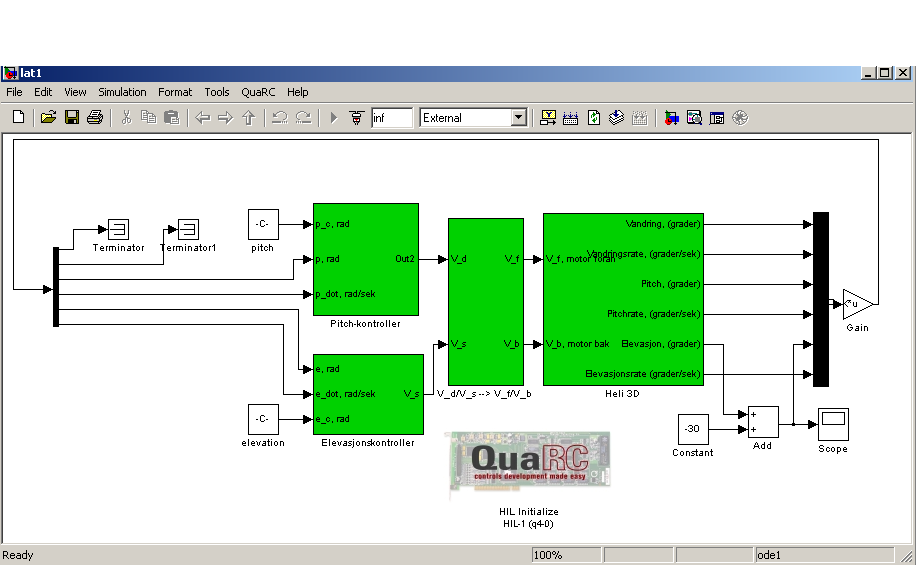
\includegraphics[width=\textwidth]{simulinkDiag.png}
	\caption{A diagram of a Simulink work flow \citep{NTNU2014}}
	\label{fig:simDiag}
\end{figure} 
%\begin{figure}[h]
%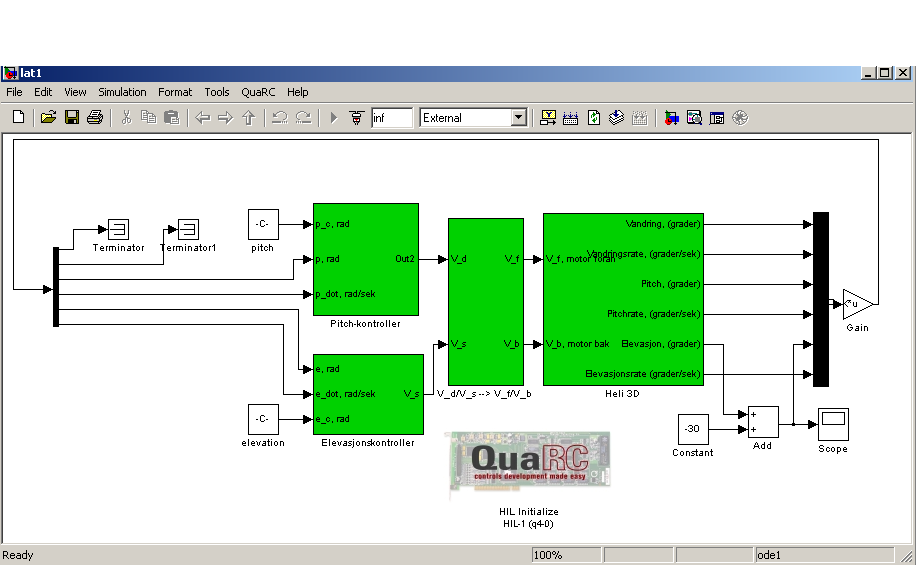
\includegraphics[\textwidth]{simulinkDiag.png}
%\caption{A diagram in Simulink.}
%\label{fig:simDiag}
%\end{figure}  
%>>>>>>> 1cbf6bd27ed03dea8337254823d98415706fdb03
%If you decide to include a figure, that's great. You can in general copy figures from the textbook, the assignement text, or other places. However: ALWAYS CITE THE SOURCE.